\section{Methods}

\subsection{Orphan origin classification}

  \subsubsection{duplicate}

    blastp or orphan genes against other coding genes in the focal species
    \cite{sun_identification_2015}. Use transitive property: if there is a
    match, and the paralog is not an orphan, assume duplication/divergence
    model. 

  \subsubsection{de novo}

    tBLASTn against nearby species. If there is a hit (50\% identity and 50\%
    coverage), and the hit is disrupted in all, classify as de novo. Manual
    checking of disruption status \cite{sun_identification_2015}.

  \subsubsection{TE}

    BLASTn against TE database (e-value cutoff of 1e-5)
    \cite{sun_identification_2015}.

\subsection{Mukherjee analysis of \textit{Leishmania major} (2015)}

  \cite{mukherjee_elucidating_2015}


  \begin{quote}

    To identify orphan gene models which are restricted to the Leishmania
    genus, we used a systematic way based on homology search. First, BLASTP
    followed by TBLASTN filtering approach ($E<10^5$ and use of low-complexity
    filters) was used against NCBI nr databases. Additionally, to further
    screen for similarity between sequences we employed Position-Specific
    Iterated BLAST (PSI-BLAST) ( Altschul et al., 1997) that can detect weaker
    homologous relationships that would otherwise be missed by the standard
    BLAST algorithms.

  \end{quote}

  The use of tBLASTn has the advantage of finding possible coding homologs of
  what would otherwise be misclassified as orphans. However, it would also
  misclassify \textit{any} true orphan that retains similarity to its
  precursor.

\subsection{Abrusan method}

Citation \cite{abrusan_integration_2013}

\textbf{Context} Orphans into networks, testing Carvunis

\textbf{Organism} Yeast

\textbf{Phylostratigraphy Procedure} 50 aa cutoff. 11 strata, 0 as Carvunis' unnanotated
genes, 1 as yeast annotated orphans, etc. Followed Carvunis methods. Time
estimates based on TimeTree.

\textbf{Protein Structure} PSSpred without homology search, since this
would introduce bias

\textbf{Aggregation propensity} Predicted with Tango

\textbf{Simulated Mutagenesis} Based on Schaefer's procedure
\cite{schaefer_protein_2010}. 1\% of the residues mutated in each of 70
steps. Mutations were introduced in context specific manner with csbuild
tool of CS-BLAST suite. At each step the secondary structure was predicted
and the percentage of sites with conserved structure was calculated.
Results were averaged for each gene across 5 replicates.

\subsection{Neme method}

Citation \cite{neme_phylogenetic_2013}

\textbf{Context} Metazoan de novo genes

\textbf{Organism} Mouse; a little human, zebrafish and stickleback

\textbf{Procedure} BLASTP(e-3) all mouse Ensembl 66 proteins against nr
database. For ps12 EST and Trace data were included in tBLASTn(e-15).
Phylostratiphy as normal.

\subsection{Hahn method}

Citation \cite{hahn_gene_2007}

\textbf{Context} 12 Drosophila genomes

\textbf{General Method} Clustering

\textbf{Notes} D. melanogaster seems to have ~2\% orphan composition. The
other genomes seem to have 10-30\% \cite{clark_evolution_2007}. Hahn
suspects this is an artefact of the overly lenient ab initio prediction
software. So he removes from the analysis all putative genes that are
unique to a single species. He calculates the percentage of Drosophila
specific genes, but since he circumsized the flange we can't really his
results to other orphan analyses. 

\textbf{Extinction} Hahn wasn't looking for, or interested in, orphans. His
focus was gene family dynamics. A very interesting result of his paper was
an estimate of family extinction. ``2,220 of the 11,434 families inferred
to have been present in the Drosophila MRCA have had such an extinction
event along at least one lineage'' pp. 7. This is something that has not
been researched nearly enough in the orphan context. If new genes are
constantly appearing, and proteome size is in equilibrium, then extinction
must be common as well. This introduces the idea of extinction
phylostratigraphy, the analysis of lineage-specific extinction events. The
technique will be more complicated than genesis phylostratigraphy since it
will require consideration of paralogs.

\subsection{Wu method}

Citation \cite{wu_novo_2011}

\textbf{Context} Finding human de novo genes

\textbf{General Method} Homology, synteny, RNA-seq, proteomics

\textbf{Details} Began with BLASTP(e-10) of all primate genomes. Removed
any proteins or splicing variants shorter than 100 amino acids (out 584).
Removed human proteins that lacked start or stop codons (weird, why were
they annotated as proteins?) (out 352). Searched these for orthologs with
BLAT against chimp and orangatan UCSC datavase. Removed all proteins for
which no homologous genomic region could be found. Removed candidates with
paralogs. Removed all if their genomic homologous region had a suitable
ORF. BLASTed remainder against mRNA database (to check for transcription)
and proteomic database (PRIDE and PeptideAtlas) to check for experimental
proof of protein product. This resulted in 27 proteins. They then ran genes
removed from the previous ann2tations, finding 33 additional true de novo
genes.

\subsection{Yang method}

Citation \cite{yang_genome-wide_2013}

\textbf{Context} Species specific and teleost specfic genes

\textbf{Organism} Zebrafish

\textbf{General method} Homology, manual

\textbf{Details} See figure.

\begin{figure}[h!]
    \centering
    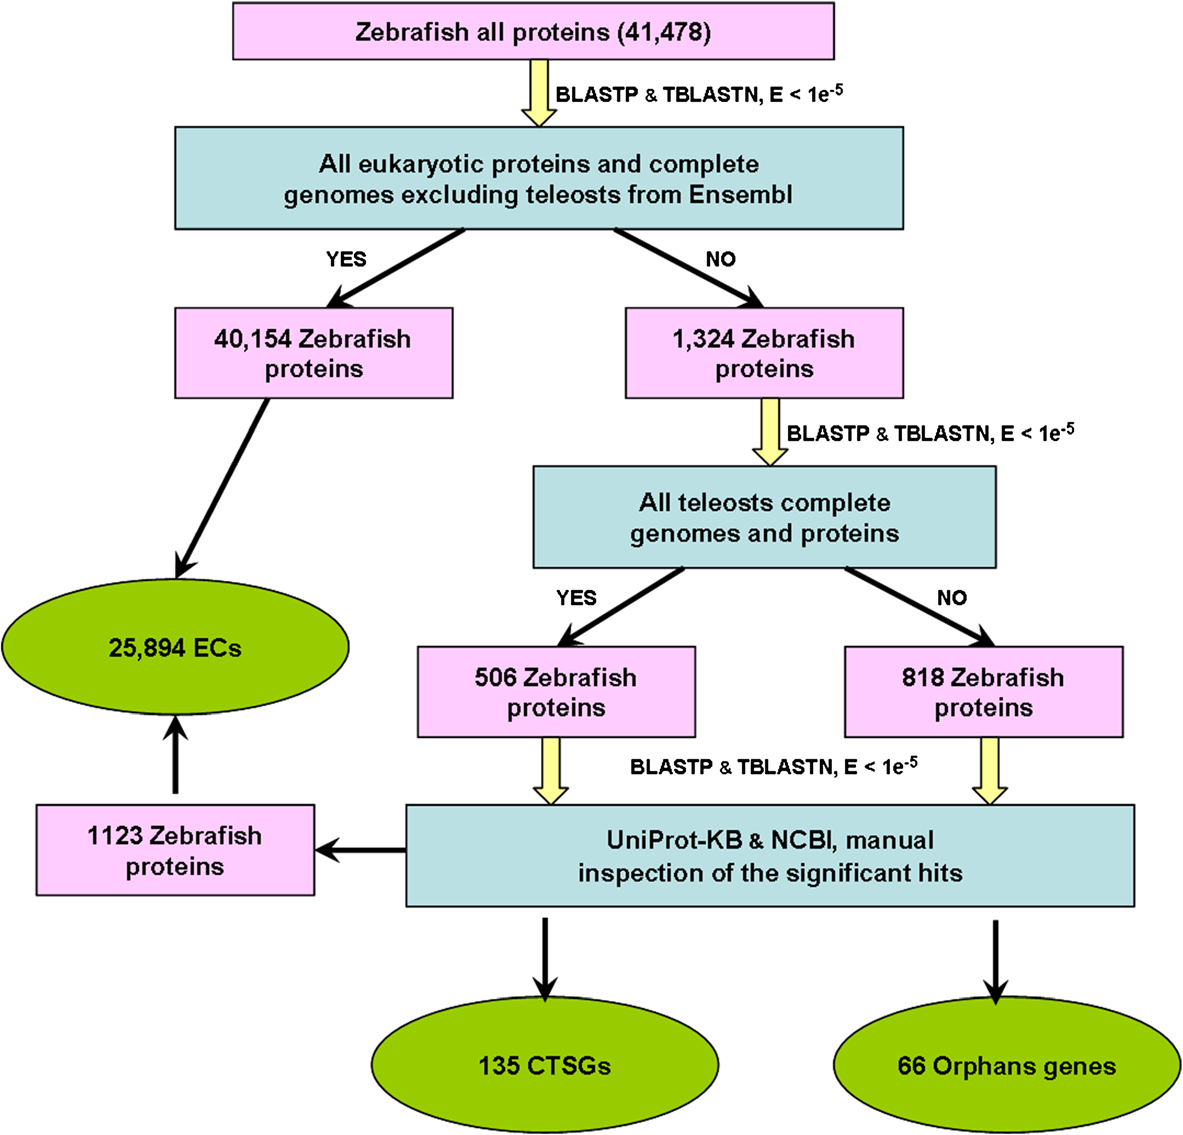
\includegraphics[scale=0.2]{yang_zebra_method}
    \caption{Yang \textit{et al.} orphan identification method}
\end{figure}
\FloatBarrier


\subsection{Toll-Reira Orphan Domain}

Citation \cite{toll-riera_emergence_2013}

\textbf{Context} Identify orphan domains in humans

\textbf{General Method} HMM

\textbf{Notes} Used PFAMs collection of domain-specific HMMs to identify
domains in all human genes. Classified domains by age group base on their
representation in 15 Eukaryotic species.
\subsection{Murphy Murine de novo genes}

Citation \cite{murphy_novo_2012}

\textbf{Context} Search for rat and mouse de novo genes

\textbf{General Method} BLAST

\textbf{Input} Rat and mouse annotated proteins (Ensembl v56)

\textbf{Procedure} BLASTP(e-3) rat-vs-mouse to identify orphans. BLASTN
rat-vs-mouse, keeping only candidates with a non-genic match (50\% coverage
and 70\% identity). Remove candidates with ortholog in non-murine species
via Ensembl compara database. Searched for potentially unannotated
protein-coding genes in opposite murine (tBLASTn to locate putative ORFs,
if translated ORF containing match aligns to at least 50\% and matches
60\%, then remove this gene). Remove an candidate lacking ATG start codon
or having an intron less than 18 bases in length. Used UniGene and Peptide
Atlas and Pride to confirm that the candidates are transcribed and
translated. BLASTed against GenBank (e-3 and 50\% coverage).

\textbf{Further Procedure} Searched for enabling mutations.

\subsection{Synteny based methods}

\subsubsection{Zhang, 2010}

Citation \cite{zhang_chromosomal_2010}

\textbf{Context} Male-biased genes in mammals

\textbf{General Method} BLAST and synteny

\textbf{Input} 
